% =====================================================================
% Readout Pseudo-Volume (RPV) -- workshop submission
% Furnace Research, 2026-06-07.
%
% Compile with pdfLaTeX. Figures live in rpv-figures/ next to this .tex;
% in Overleaf, upload the rpv-figures/ directory alongside this file.
% Self-contained: inline thebibliography (no .bib) and the summary table
% is \input from rpv-figures/table1_summary.tex (emitted by the figure
% builder). Preamble mirrors the ACE (PRI v4) draft for portability.
%
% Method name "Readout Pseudo-Volume (RPV)" locked 2026-06-07. Internal
% exploratory slug: shadow-ambiguity / candidate #10.
% Pre-registered protocol: PRE_REGISTRATION_DRAFT.md v2 (t0 repo,
% exploratory/shadow-ambiguity/). Fresh seed 20260611 (pilot seed
% 20260607 not reused). Figures + numbers: comprehensive_outputs/.
%
% Revision 2026-06-09: framing only. Leads with the confidence-independent
% positive and reads the null_ratio overlap as convergent validation of a
% real commit-time geometry; foregrounds the Delta-h-free / centered-Fisher
% formulation; names the symmetric-increment + fair-base collapse-cohort
% follow-up. All numbers and the registered H1 NO-GO verdict are UNCHANGED.
% =====================================================================

\documentclass[10pt, letterpaper]{article}

\usepackage[margin=1in]{geometry}
\usepackage[T1]{fontenc}
\usepackage{microtype}
\usepackage{lmodern}
\usepackage{amsmath, amssymb, amsthm}
\usepackage{booktabs}
\usepackage{graphicx}
\usepackage{xcolor}
\usepackage{natbib}
\usepackage[hidelinks]{hyperref}
\usepackage[capitalise]{cleveref}
\usepackage{caption}
\usepackage{enumitem}
\usepackage{authblk}
\usepackage{placeins}

\setlength{\parskip}{0.4em}
\setlength{\parindent}{0pt}
\setlength{\textfloatsep}{0.8em plus 0.2em minus 0.2em}
\setlength{\floatsep}{0.8em plus 0.2em minus 0.2em}
\renewcommand{\topfraction}{0.95}
\renewcommand{\bottomfraction}{0.9}
\renewcommand{\textfraction}{0.05}
\renewcommand{\floatpagefraction}{0.8}
\setcounter{topnumber}{3}
\setcounter{bottomnumber}{2}
\setcounter{totalnumber}{5}

% Convenience macros
\newcommand{\auroc}{\text{AUROC}}
\newcommand{\Fc}{F_{c}}
\newcommand{\Wu}{W_{u}}
\newcommand{\pmax}{p_{\max}}
\newcommand{\effrank}{\textsf{fisher\_eff\_rank}}
\newcommand{\spent}{\textsf{spectral\_entropy}}
\newcommand{\logvol}{\textsf{shadow\_logvol}}
\newcommand{\nullr}{\textsf{null\_ratio}}

\title{Readout Pseudo-Volume: A Confidence-Independent,\\
$\Delta h$-Free Commitment Signal That Converges with a Prior Detector}

\author{Michael S.R. Kitti \\ \texttt{msrkittty@proton.me}}

\date{Workshop submission, 2026-06-07 \quad (revised 2026-06-09)}

\begin{document}

\maketitle

\begin{abstract}
When a language model commits to an answer token, its hidden state is
read out through the unembedding $\Wu$ and collapsed to a single token.
We introduce \textbf{Readout Pseudo-Volume (RPV)}: the eigen-spectrum
of the centered softmax-Fisher pullback of that readout map at the
commit instant, summarized by its effective rank and off-top
log-pseudo-volume. RPV is a property of the readout metric itself---the
exact categorical Fisher, not an uncentered surrogate---and is
independent of the commit motion $\Delta h$, so it reads commitment
geometry from a single state with no per-step motion trace and none of
the step-0 $\Delta h$ fragility of earlier signals.

We evaluate RPV under a protocol pre-registered before the reported run:
13 open-weight models, two benchmarks (ANLI~R1, TriviaQA; 26
model--benchmark pairs), with fair baselines and brittleness,
multiplicity, and family-spanning gates. RPV is a genuinely
confidence-independent commitment signal---it beats plain confidence by
a random-effects meta increment of $+0.102$ $\auroc$ (95\% CI
$[+0.065,+0.140]$; $p\approx 5\times10^{-8}$), with per-pair positives
spanning three model families. It is not confidence in disguise.

We then ask the question new commit-moment signals are rarely asked:
does RPV add information beyond a \emph{prior detector of our own}---the
Fisher-based \nullr{} (PRI~v3)? Although the two are built from
different objects (a $\Delta h$-independent centered spectrum versus a
projection of one specific $\Delta h$), RPV recovers nearly the same
discriminative content: its increment over a baseline that already
contains \nullr{} is $+0.011$, below the pre-registered $+0.02$ minimum
effect, so the primary gate is \textbf{NO-GO}. We read this convergence
of two independently constructed statistics as evidence that the
commit-time geometry is \emph{real}, not as a defeat---and RPV adds
genuine power exactly where \nullr{} collapses (regime slope $+0.080$).
RPV is thus a confidence-independent, $\Delta h$-free reading of the
commit-time readout that coincides with an existing detector on most
models and backstops it where that detector fails; we register the
symmetric-increment and fair-base collapse-cohort tests that would
establish whether it is the more general of the two.
\end{abstract}

% =====================================================================
\section{Introduction}
% =====================================================================

Large language models are increasingly deployed where a confidently
stated but unsupported answer is costly, making the detection of such
failures a practical safety and debugging problem. One promising,
single-pass approach reads a signal not from the model's output text
but from its internal state at the moment it commits to the first
answer token---in contrast to methods that resample many generations
\citep{farquhar2024semantic, kitti2026commitment}. A reliable
commit-moment signal would flag unsupported answers at the cost of a
single forward pass, which is attractive for deployment-time
monitoring.

This commit-moment program has already produced several
representation-space signals at generation step~1. The Predictive
Rupture Index (PRI) family progressed from a cosine rupture (v1) to a
Fisher pullback distance (v2) to \nullr{} (v3), the fraction of the
commit motion $\Delta h$ lying off the top singular directions of
$\sqrt{\mathrm{diag}(p)}\,\Wu$; a companion line reads the same instant
from $\Wu$-free attention features \citep{kitti2026pri,
kitti2026priv2}. Grounded in information geometry on the probability
simplex \citep{amari2016information}, these signals establish that the
commit instant carries discriminative structure---and that the useful
cell must be calibrated per model and distribution.

As such signals proliferate, however, each is typically validated in
only two ways: that it beats chance against labels, and that it is not
merely a restatement of the model's confidence. They are rarely tested
against \emph{one another}. This leaves a basic interpretability
question open: when a new commit-moment statistic discriminates, is it
carrying \emph{new} information about the model's commitment, or
re-describing structure an existing detector already captures? The gap
is one of signal \emph{redundancy and validity}, not benchmark
coverage---and it is exactly where interpretability claims demand
care, separating ``the model has commitment structure'' from ``this
statistic adds information beyond existing probes.''

We address this for one concrete, well-motivated candidate: the
geometry of the readout map itself. The committed token is the
\emph{shadow} of the hidden state $h$; because $z=\Wu h$ is injective
when the vocabulary exceeds the hidden width, no information is lost in
the linear readout, and the collapse to a single token happens entirely
in $\mathrm{softmax}$ and $\arg\max$, whose local geometry is the
centered softmax-Fisher metric pulled back to hidden space. We
introduce \textbf{Readout Pseudo-Volume (RPV)}: the eigen-spectrum of
that metric---its effective rank and off-top log-pseudo-volume.
Crucially, RPV is a property of the metric and is independent of any
particular motion $\Delta h$, whereas \nullr{} measures a specific
$\Delta h$; the two could be orthogonal or redundant, which we test
directly by placing \nullr{} in the baseline.

We study whether RPV adds a commitment signal beyond confidence and
beyond \nullr{} across 13 open-weight models on ANLI~R1 and TriviaQA,
under a protocol pre-registered before the reported run. RPV is
genuinely confidence-independent (random-effects meta increment
$+0.102$ $\auroc$ over confidence, three families). Against our own
prior \nullr{} detector it does not clear the pre-registered
incremental bar (increment $+0.011$ over a baseline that already
contains \nullr{}, below $+0.02$; H1 \textbf{NO-GO}): two statistics
built from different objects converge on the same commit-time
structure---which we read as validation that the structure is real, and
which leaves RPV a genuine backstop exactly where \nullr{} collapses.
The broader lesson is constructive: confidence-independence is necessary
but not sufficient evidence that an interpretability signal is new, so
new commit-moment signals should be benchmarked against prior detectors,
not confidence alone. We contribute (i) RPV, a $\Delta h$-independent
readout-geometry statistic built on the centered categorical Fisher, and
its formal relation to \nullr{} (\cref{sec:method}); (ii) a
pre-registered, redundancy-aware evaluation with fair baselines and
brittleness, multiplicity, and family-spanning gates, plus a released
JSON-only analysis harness (\cref{sec:eval}); and (iii) a convergent
negative---RPV recovers a prior detector rather than beating it---together
with the symmetric-increment and collapse-cohort tests that would
establish whether the $\Delta h$-free formulation is the more general of
the two (\cref{sec:results}).

% =====================================================================
\section{Readout Pseudo-Volume}
\label{sec:method}
% =====================================================================

\paragraph{Setup.}
At generation step~1 let $h\in\mathbb{R}^d$ be the post-final-norm
hidden state, $\Wu\in\mathbb{R}^{V\times d}$ the unembedding,
$z=\Wu h$, $p=\mathrm{softmax}(z)$, and the committed token
$\arg\max_i p_i$. With $V\gg d$ and generic $\Wu$, $h\mapsto z$ has
full column rank and is injective; the lossy steps are
$\mathrm{softmax}$ and $\arg\max$, not $\Wu$.

\paragraph{The centered softmax-Fisher pullback.}
The Fisher information of the categorical in logit coordinates is
$F_z=\mathrm{diag}(p)-pp^{\top}$, the Hessian of
$\mathrm{KL}(p_z\,\|\,p_{z+\delta})$ at $\delta=0$. Pulling back through
$z=\Wu h$ gives the $d\times d$ PSD metric
\begin{equation}
\Fc \;=\; \Wu^{\top}\!\big(\mathrm{diag}(p)-pp^{\top}\big)\,\Wu .
\end{equation}
For a hidden perturbation $\delta h$ with $\zeta=\Wu\,\delta h$,
\begin{equation}
\mathrm{KL}\big(p_h\,\|\,p_{h+\delta h}\big)\approx
\tfrac12\,\delta h^{\top}\Fc\,\delta h
=\tfrac12\,\mathrm{Var}_p(\zeta),
\end{equation}
so $\Fc$ measures how loudly each direction of hidden motion shows up
in the output distribution.

\paragraph{Statistics (functions of the spectrum).}
Eigendecompose $\Fc=\sum_i\lambda_i v_iv_i^{\top}$ with
$\lambda_1\ge\cdots\ge0$, take the active set
$\{\lambda_i>\texttt{rel\_tol}\cdot\lambda_{\max}\}$, normalize
$\tilde\lambda_i=\lambda_i/\sum_j\lambda_j$, and let
$H=-\sum_i\tilde\lambda_i\log\tilde\lambda_i$. We register:
\begin{itemize}[leftmargin=1.4em, itemsep=2pt, topsep=2pt]
\item \effrank${}=\exp(H)$ (Roy--Vetterli effective rank): how many
directions the readout resolves. \textbf{Scale-invariant}---it depends
on spectral \emph{shape}, not magnitude. \textbf{(Primary.)}
\item \spent${}=H/\log(\mathrm{rank}_{\mathrm{eff}})\in[0,1]$:
monotone-equivalent to effective rank. \textbf{(Secondary.)}
\item $\logvol_r=-\tfrac{1}{2(d-r)}\sum_{i>r}\log(\lambda_i+\varepsilon)$,
the off-top log-pseudo-volume of the KL-ellipsoid---``how far can $h$
move in non-decision directions without changing the shadow.'' Pinned
at $r=1$ (top-1 = commit axis); entered as
$\textsf{neg\_shadow\_logvol\_r1}=-\logvol_1$. \textbf{(Secondary.)}
\end{itemize}

\paragraph{Confidence versus commitment.}
Confidence is the \emph{scale} of $\Fc$: as $p\to$ one-hot,
$\mathrm{diag}(p)-pp^{\top}\to0$ and the whole spectrum shrinks.
Commitment-quality is the \emph{shape} of the spectrum. The two are
correlated but distinct, which is why the primary is a scale-invariant
shape statistic and why we add explicit confidence controls
(\cref{sec:eval}).

\paragraph{Relation to \nullr{} (v3).}
This is the crux of the redundancy question. \nullr{} uses the
\emph{uncentered} surrogate $A=\sqrt{\mathrm{diag}(p)}\,\Wu$ and reports
the Euclidean fraction of a \emph{specific} commit motion $\Delta h$
lying outside the top-$r$ right-singular directions of $A$. RPV instead
reads the eigen-spectrum of the \emph{centered} $\Fc$---a
$\Delta h$-independent property of the readout metric, not a projection
of one motion vector. The two could, in principle, be orthogonal;
whether they are is an empirical question we pre-register.

\paragraph{Aggregation and computation.}
Statistics are read at the readout and at late blocks via the logit
lens $p_\ell=\mathrm{softmax}(\Wu\cdot\mathrm{norm}(h_\ell))$. We pin
the late window with no best-layer selection: for $B$ blocks, the late
count is $\lceil B/4\rceil$ and the aggregate is the arithmetic mean
over blocks $[B-\lceil B/4\rceil,\dots,B-1]$ plus the readout. The
spectrum is computed by a $K{\times}K$ dual on the top-$K$ probability
support ($K{=}512$); a contract suite (7/7) verifies the temperature
identity, the degeneracy limit, the $h$-space-versus-vocab distinction,
and agreement with the production eigendecomposition.

% =====================================================================
\section{Pre-Registered Evaluation}
\label{sec:eval}
% =====================================================================

The protocol below was written down (\texttt{PRE\_REGISTRATION\_-
DRAFT.md} v2) before the reported run, which used a fresh held-out seed
(20260611; the pilot seed 20260607 was explicitly not reused) with code
and data hashes recorded. This is the exploratory morphology lab's
pre-registration: it applies the same anti-self-deception discipline as
our sealed line \citep{nosek2018preregistration,
pineau2021reproducibility} but is reported as a pre-registered protocol,
not a formally sealed gate.

\paragraph{Hypotheses and bars.}
\textbf{H1 (primary).} The oriented primary statistic \effrank{} adds
incremental AUROC over \emph{both} fair bases in a
cross-(model, benchmark) random-effects meta-analysis: base~A
$=\{\textsf{surprise}\}$ and base~B
$=\{\textsf{surprise},\nullr{},\pmax\}$. The meta mean must reach a
minimum practical effect of $+0.02$; a CI excluding zero is necessary
but not sufficient. \textbf{H2 (secondary).} The increment over
$\{\textsf{surprise},\nullr{}\}$ is larger where \nullr{} is weak,
weakness defined as $1-\auroc(\nullr{},\text{train-locked})$. The
candidate is falsified if the base-A meta CI includes 0, if the effect
lives only at high brittleness, if it fails multiplicity, or if the
meta effect is below $+0.02$.

\paragraph{Discipline.}
Orientation is locked from pre-registration or train folds only (never
test labels). The brittleness gate discards a claim if either
$\mathrm{corr}(\text{stat},\pmax)$ or
$\mathrm{corr}(\text{stat},\textsf{surprise})$ has bootstrap upper CI
$\ge 0.75$ at the exact pinned aggregate. Multiplicity: exactly one
uncorrected primary; all other statistics/endpoints form a Holm-
corrected family. A general claim requires per-pair positives (clearing
both bases at $\ge 0.02$, lower CI $>0$) in $\ge 2$ collapse-regime
models spanning $\ge 2$ architecture families; a Qwen-only pass would
license only a ``Qwen-family \nullr{} rescue'' claim. Controls:
shuffled-label null (1000 permutations), a random-rotation
\emph{invariance} check (spectral statistics must be unchanged under a
Householder reflection in hidden coordinates), a degraded-base flag,
and a label-free temperature pre-check.

\paragraph{Data and estimation.}
13 open-weight 4-bit MLX models \citep{mlxframework} spanning 5
families (llama, mistral, qwen, phi, gemma) $\times$ 2 benchmarks (ANLI~R1
$n{=}200$; TriviaQA paired $n{=}100$) yield 26 completed pairs
(gpt-oss-20b skipped, too heavy for the local cache). The commit instant
is generation step~1; features are
$\{\textsf{label},\textsf{surprise},\pmax,\nullr{},\effrank{},
\textsf{neg\_shadow\_logvol\_r1},\spent{}\}$. We use repeated 5-fold
out-of-fold logistic regression ($\ge 10$ repeats, averaged OOF
probabilities, shared fold assignments across feature sets), paired
bootstrap CIs ($n_{\text{boot}}{=}10{,}000$), and a random-effects meta
(DerSimonian--Laird; modified Knapp--Hartung $t$ retained for small-$k$
honesty).

% =====================================================================
\section{Results}
\label{sec:results}
% =====================================================================

\subsection{RPV beats plain confidence}

Over base~A $\{\textsf{surprise}\}$, \effrank{} adds a random-effects
meta increment of $\mathbf{+0.102}$ $[+0.065,+0.140]$ AUROC
($k{=}26$, $p\approx 5\times10^{-8}$; the more conservative
Knapp--Hartung interval is $[+0.060,+0.145]$). \Cref{fig:forest} shows
the per-pair distribution: the effect is broadly positive, with
per-pair positives spanning three families (llama, mistral, qwen). The
brittleness gate passes (no upper CI $\ge 0.75$), and oriented partial
correlations beyond confidence are nonzero (e.g.\
$\textsf{neg\_shadow\_logvol\_r1}$ partial $r\approx-0.46$ controlling
for surprise). RPV is therefore a genuinely confidence-independent
commitment signal---not surprise in disguise.

\begin{figure}[!htbp]
  \centering
  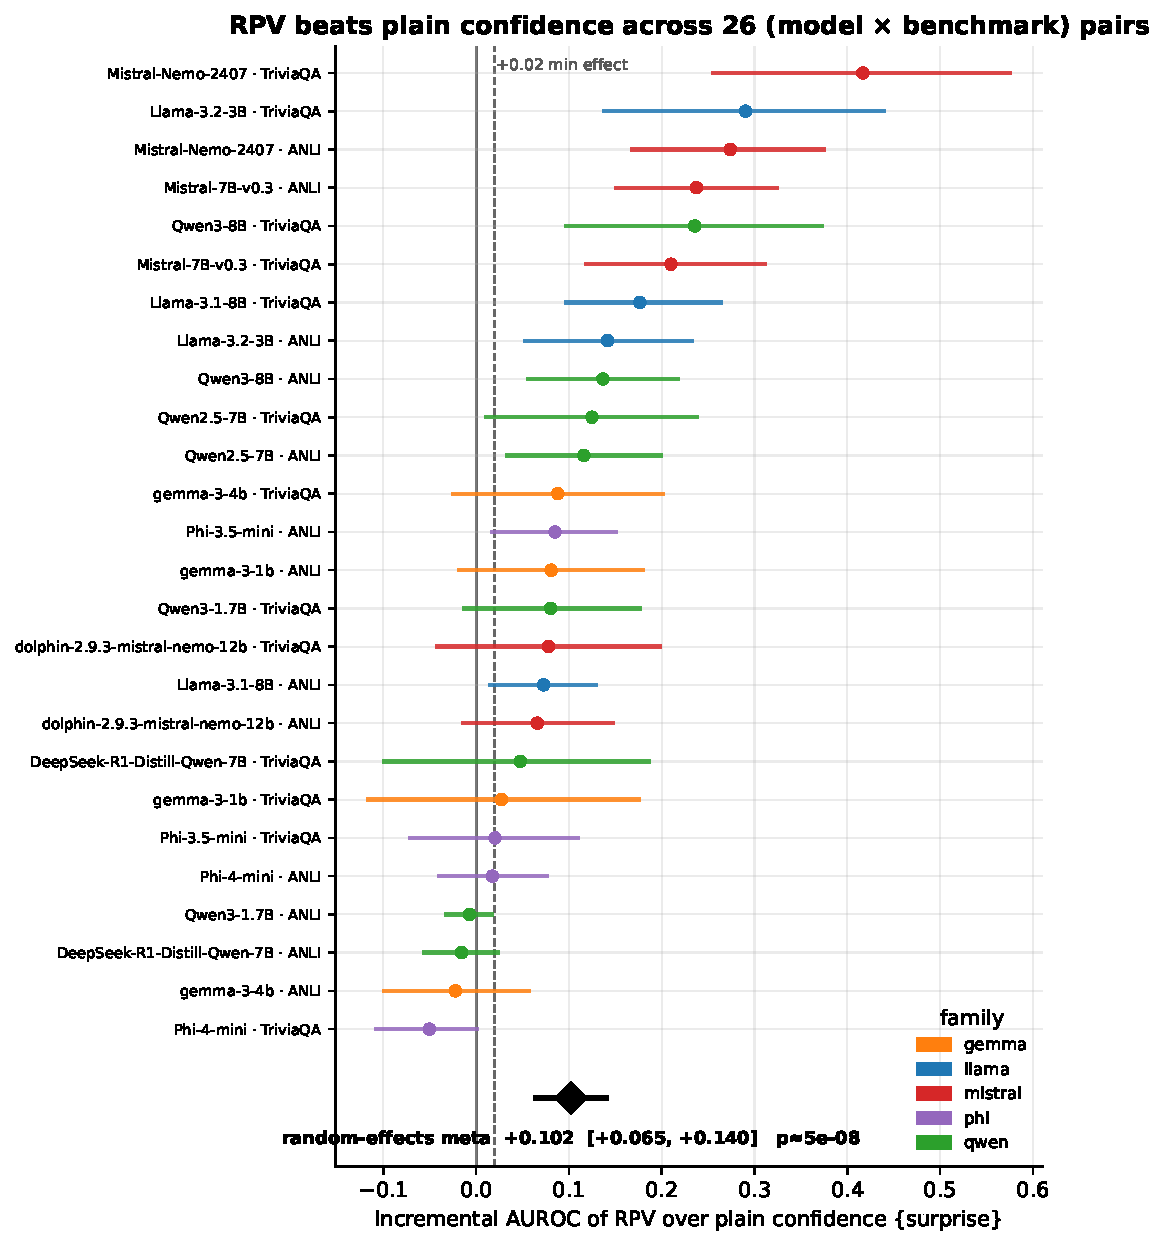
\includegraphics[width=0.82\linewidth]{rpv-figures/fig1_forest_rpv_vs_confidence.pdf}
  \caption{RPV (\effrank{}) incremental AUROC over plain confidence
  $\{\textsf{surprise}\}$ for each of the 26 (model $\times$ benchmark)
  pairs, colored by family, with the random-effects meta diamond.
  Dashed line is the pre-registered $+0.02$ minimum effect. RPV beats
  confidence broadly: meta $+0.102$ $[+0.065,+0.140]$,
  $p\approx 5\times10^{-8}$.}
  \label{fig:forest}
\end{figure}

\subsection{RPV converges with \nullr{} (H1 NO-GO)}

The picture inverts once the existing detector enters the baseline.
\Cref{fig:ladder} shows the meta increment as \nullr{} (and then
$\pmax$) join the base: $+0.102 \to +0.027 \to \mathbf{+0.011}$. The
base-B increment of $+0.011$ sits \emph{below} the pre-registered
$+0.02$ minimum practical effect (and its small-$k$ Knapp--Hartung
interval crosses zero), so the registered H1 gate is
\textbf{NO-GO}---even though base-A and base-B DerSimonian--Laird CIs
both exclude zero and the family-spanning rule is satisfied.
\Cref{tab:rpv_summary} collects the verdict. The honest reading is also
the encouraging one: on most models the centered spectrum and \nullr{}'s
off-axis projection track the \emph{same} commitment structure, so two
independently constructed statistics corroborate that the commit-time
geometry is real rather than an artifact of either construction.

\begin{figure}[!htbp]
  \centering
  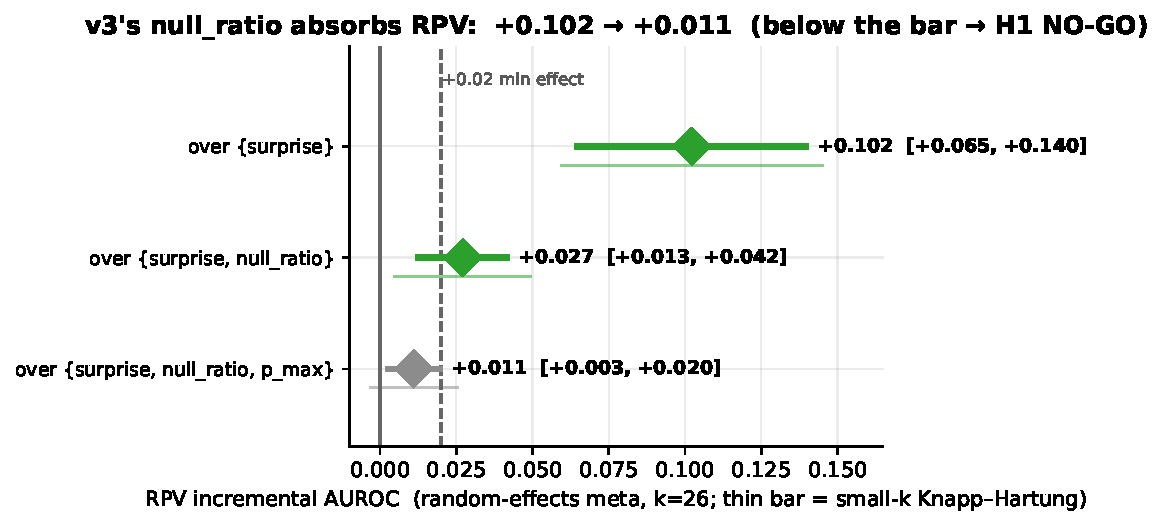
\includegraphics[width=0.86\linewidth]{rpv-figures/fig2_redundancy_ladder.pdf}
  \caption{Redundancy ladder: the RPV meta increment as the baseline
  grows. Adding \nullr{} absorbs most of the signal
  ($+0.102\to+0.027$); adding $\pmax$ leaves $+0.011$, below the
  $+0.02$ bar (grey; thin bar = small-$k$ Knapp--Hartung). This is the
  registered H1 NO-GO.}
  \label{fig:ladder}
\end{figure}

\begin{table}[!htbp]
  \centering
  \caption{Pre-registered verdict summary (random-effects meta,
  $k{=}26$ pairs). RPV clears base~A but not base~B's $+0.02$ bar;
  brittleness and family-spanning pass, but the registered H1 gate is
  NO-GO. H2 regime slope is positive.}
  \label{tab:rpv_summary}
  \small
  \input{rpv-figures/table1_summary.tex}
\end{table}

\subsection{RPV complements \nullr{} where it collapses}

The one place RPV earns incremental power is exactly \nullr{}'s blind
spot. \Cref{fig:complement} regresses RPV's increment over
$\{\textsf{surprise},\nullr{}\}$ on \nullr{} weakness: the weighted
slope is $\mathbf{+0.080}$, and the largest gains are on Qwen3-8B---the
model where \nullr{} sits at chance---where RPV adds double-digit
AUROC. Consistent with a real-but-overlapping signal, 28 of 234
secondary/per-pair tests survive Holm correction (12
\textsf{neg\_shadow\_logvol}, 9 \effrank{}, 7 \spent{}), concentrated
in \nullr{}-weak pairs. The signal is real; it is mostly \nullr{}-
shaped.

\begin{figure}[!htbp]
  \centering
  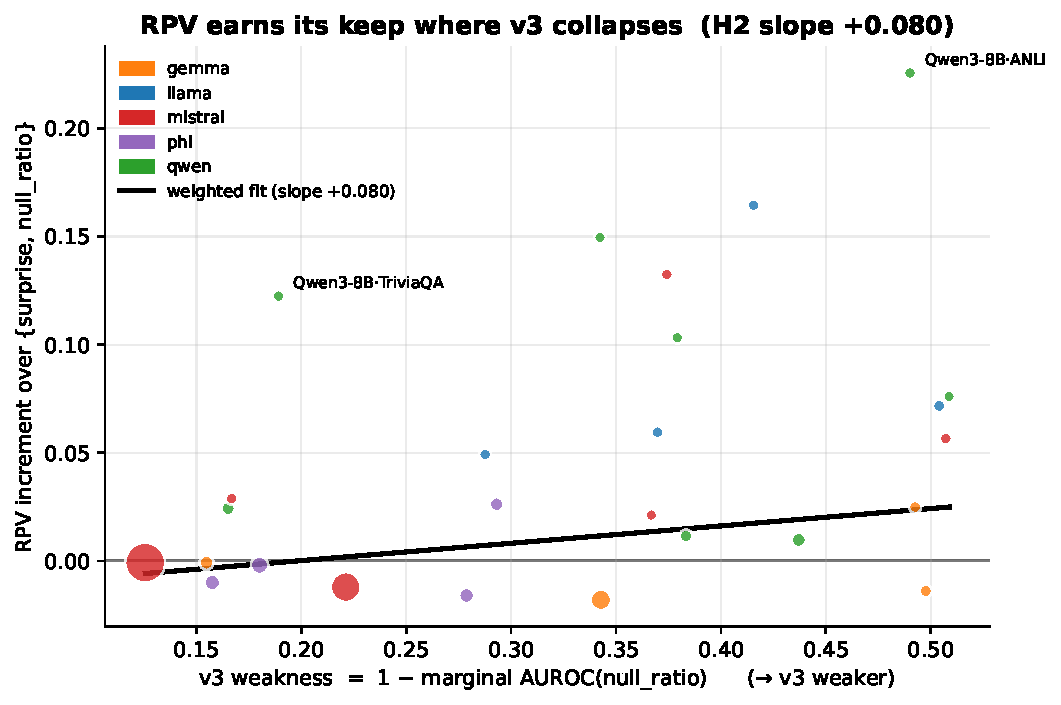
\includegraphics[width=0.86\linewidth]{rpv-figures/fig3_collapse_complement.pdf}
  \caption{H2: RPV increment over $\{\textsf{surprise},\nullr{}\}$
  versus \nullr{} weakness ($1-\auroc(\nullr{})$); point size $\propto$
  inverse variance. RPV adds most where \nullr{} is weakest (weighted
  slope $+0.080$); Qwen3-8B is the standout.}
  \label{fig:complement}
\end{figure}

% =====================================================================
\FloatBarrier
\section{Discussion}
% =====================================================================

\paragraph{What the convergence means.}
RPV and \nullr{} are constructed from different objects---a
$\Delta h$-independent centered spectrum versus the off-axis projection
of a specific commit motion through an uncentered surrogate---yet they
carry nearly the same discriminative content on most models. We read
this as convergent validation: when two statistics built from different
constructions agree, the most parsimonious explanation is that the
commitment structure they both detect is real and lives in a shared
low-dimensional readout geometry---when the readout resolves few
directions (low effective rank, large pseudo-volume), the commit motion
also tends to fall off the lit decision axis. The overlap is
\emph{symmetric}: on this cohort neither statistic subsumes the other,
so the honest verdict is convergence, not a successor relation in either
direction. Which (if either) is the more general object is an empirical
question we have not answered here; the $\Delta h$-free construction
makes RPV the more principled \emph{candidate}, but candidacy is not the
test (see ``The open thread'').

\paragraph{The open thread.}
The positive H2 slope and the Qwen3-8B gains suggest a concrete, narrow
use: RPV as a backstop where \nullr{} collapses. Two pre-registered
tests would settle whether RPV is merely a backstop or genuinely the
more general object. First, the \emph{symmetric increment}: measure
\nullr{}'s gain over $\{\textsf{surprise},\effrank{}\}$, the mirror of
the ladder we ran; subsumption requires not only that \nullr{} absorbs
RPV but that RPV absorbs \nullr{}, and only the first direction has been
tested. Second, a \emph{fair-base collapse cohort}: pre-register a panel
of \nullr{}-failure models (Qwen3-8B-like) and score RPV's increment
over the fair $\{\textsf{surprise}\}$ base, since the apparent
double-digit Qwen3-8B gain shrank to $+0.044$ $[-0.025,+0.111]$ once the
degraded base was corrected (below). If RPV adds on a fair base across
that cohort \emph{and} \nullr{} fails to absorb RPV in the symmetric
test, the $\Delta h$-free formulation earns ``more general''---sealed,
not narrated. We register this as open, not validated.

\paragraph{Relation to the wider line.}
RPV is the $\Wu$-using readout sibling of the $\Wu$-free ACE attention
panel; both pass discriminability against confidence and both require
per-model calibration. Together with the v1/v2/v3 progression
\citep{kitti2026pri, kitti2026priv2, kitti2026commitment} and the
information-geometric view of the simplex \citep{amari2016information},
the consistent finding is that commit-moment signals are real but
neither universal across models nor mutually orthogonal.

\paragraph{The gauntlet, and the inflation it caught.}
A pilot reported a $+0.13$ increment on Qwen3-8B. Adversarial review
found it was measured over a \emph{degraded} base
($\{\textsf{surprise},\nullr{}\}$ had fallen below surprise alone
because \nullr{} was sub-chance on that model); recomputed over the
fair $\{\textsf{surprise}\}$ base the named statistics had CIs crossing
zero ($+0.044$ $[-0.025,+0.111]$). The fair-base requirement,
brittleness gate, family-spanning rule, and shuffled-label null exist
to catch exactly this, and they turned a hopeful positive into the
honest negative reported here.

\paragraph{Limitations.}
4-bit MLX quantization (uniform across the panel); two benchmarks;
per-model $n$ of 100--200 is underpowered, which is why the claim is
meta-analytic rather than per-model; and ``redundant with \nullr{}''
is the empirical verdict on this cohort, not a guarantee for unseen
distributions.

% =====================================================================
\section{Conclusion}
% =====================================================================

Readout Pseudo-Volume is a clean, $\Delta h$-independent reading of the
readout map's geometry at the commit moment, built on the exact
categorical Fisher. Under a pre-registered cross-model test it is
genuinely confidence-independent and beats plain confidence by a
comfortable meta margin. Measured against our own prior \nullr{}
detector it converges rather than exceeds---it does not clear the
incremental bar over a baseline that already contains \nullr{} (H1
NO-GO), except in that detector's collapse regime---and we read that
convergence of two independently constructed statistics as evidence that
the commit-time geometry is real. The same discipline that would have
let us overclaim a degraded-base ``rescue'' instead leaves us with a
sharper and more useful result: a confidence-independent, $\Delta h$-free
commitment signal that corroborates an existing detector, backstops it
where it collapses, and comes with a pre-registered path---the symmetric
increment and a fair-base collapse cohort---to test whether the
$\Delta h$-free formulation is the more general of the two.

% =====================================================================
% References (inline; author-year keys match \citep calls)
% =====================================================================
\begin{thebibliography}{99}

\bibitem[Amari(2016)]{amari2016information}
S.-i. Amari.
\newblock \emph{Information Geometry and Its Applications}.
\newblock Applied Mathematical Sciences, Vol.~194. Springer, 2016.

\bibitem[Farquhar et al.(2024)]{farquhar2024semantic}
S.~Farquhar, J.~Kossen, L.~Kuhn, and Y.~Gal.
\newblock Detecting Hallucinations in Large Language Models Using
Semantic Entropy.
\newblock \emph{Nature}, 630:625--630, 2024.

\bibitem[Kitti(2026a)]{kitti2026pri}
M.~S.~R. Kitti.
\newblock Predictive Rupture as a Signal for Hallucination Detection
in Large Language Models.
\newblock Furnace Research preprint, 22~January 2026.

\bibitem[Kitti(2026b)]{kitti2026commitment}
M.~S.~R. Kitti.
\newblock Hallucinations Rupture at Commitment, Not at Encoding.
\newblock Furnace Research preprint, 17~March 2026.

\bibitem[Kitti(2026c)]{kitti2026priv2}
M.~S.~R. Kitti.
\newblock Fisher-Pullback Predictive Rupture Index Detects
Commitment-Time Strain Across Decoder Architectures.
\newblock Furnace Research preprint, 9~April 2026.

\bibitem[Nosek et al.(2018)]{nosek2018preregistration}
B.~A. Nosek, C.~R. Ebersole, A.~C. DeHaven, and D.~T. Mellor.
\newblock The preregistration revolution.
\newblock \emph{PNAS}, 115(11):2600--2606, 2018.

\bibitem[Pineau et al.(2021)]{pineau2021reproducibility}
J.~Pineau, P.~Vincent-Lamarre, K.~Sinha, et al.
\newblock Improving Reproducibility in Machine Learning Research.
\newblock \emph{JMLR}, 22(164):1--20, 2021.

\bibitem[Apple ML Research(2023)]{mlxframework}
Apple ML Research.
\newblock MLX: An array framework for Apple Silicon.
\newblock GitHub repository, 2023--present. Companion \texttt{mlx-lm}
provides the 4-bit-quantized checkpoints used here.

\end{thebibliography}

% =====================================================================
\appendix

\section{Reproducibility}
\label{app:repro}
Pre-registered protocol: \texttt{PRE\_REGISTRATION\_DRAFT.md} v2
(exploratory/shadow-ambiguity/, t0-morphology-furnace). Fresh seed
20260611; pilot seed 20260607 not reused; code and data SHA-256 hashes
recorded per pair. Figures and the summary table are regenerated from
\texttt{comprehensive\_outputs/} (26 per-pair JSONs + meta) by
\texttt{paper/figures/build\_all.sh}---JSON only, no model re-traces.

\section{Controls (label-free and invariance)}
\label{app:controls}
A label-free temperature pre-check confirmed all four statistics are
not pure confidence proxies ($|\rho|<0.9$ versus surprise across
generic-text commits on four models; the most-decoupled was Qwen3-8B).
A random Householder reflection in hidden coordinates left the spectral
statistics unchanged to numerical tolerance ($<2\times10^{-9}$
max-abs delta), confirming the registered statistics are rotation
invariances rather than coordinate artifacts. The full 26-pair table,
the 7/7 contract suite, and the shuffled-label null are in the
supplementary material.

\end{document}
